\begin{table}[h]
    \centering
    \caption{Comparação do Tempo do Insertion Sort}
    \begin{tabular}{|c|c|c|c|c|c|c|}
        \hline
        Tamanho de Entrada & 10 & 100 & 1000 & 10000 & 100000 & 1000000 \\
        \hline
        Crescente & 0.000000 & 0.000000 & 0.000000 & 0.000000 & 0.008000 & 0.100000 \\
        \hline
        Decrescente & 0.000000 & 0.000000 & 0.000000 & 0.001000 & 0.008000 & 0.099000 \\
        \hline
        Aleatória & 0.000000 & 0.000000 & 0.000000 & 0.001000 & 0.014000 & 0.173000 \\
        \hline
    \end{tabular}
    \label{tab:comparacao}
\end{table}

A Tabela mostra o Merge Sort nos 6 diferentes tamanhos de entrada e 3 situações diferentes de como as entradas são postas em determinados arquivos, assim como os demais algoritmos. Os resultados evidenciaram certas características fundamentais do algoritmo Merge Sort. Este algoritmo exibe uma performance uniforme e estável, gerando resultados semelhantes em diversas condições de entrada. O Merge Sort, devido à sua abordagem de divisão e conquista, mantém uma performance consistente, independentemente do estado inicial dos dados. Isso o torna eficiente tanto para dados ordenados quanto para dados parcialmente ordenados. Em média, o Merge Sort mantém uma complexidade de tempo O(n log n), tornando-o uma escolha sólida para ordenação em cenários de grande escala e em diferentes configurações de dados.

 \begin{figure}[H]
    \centering
    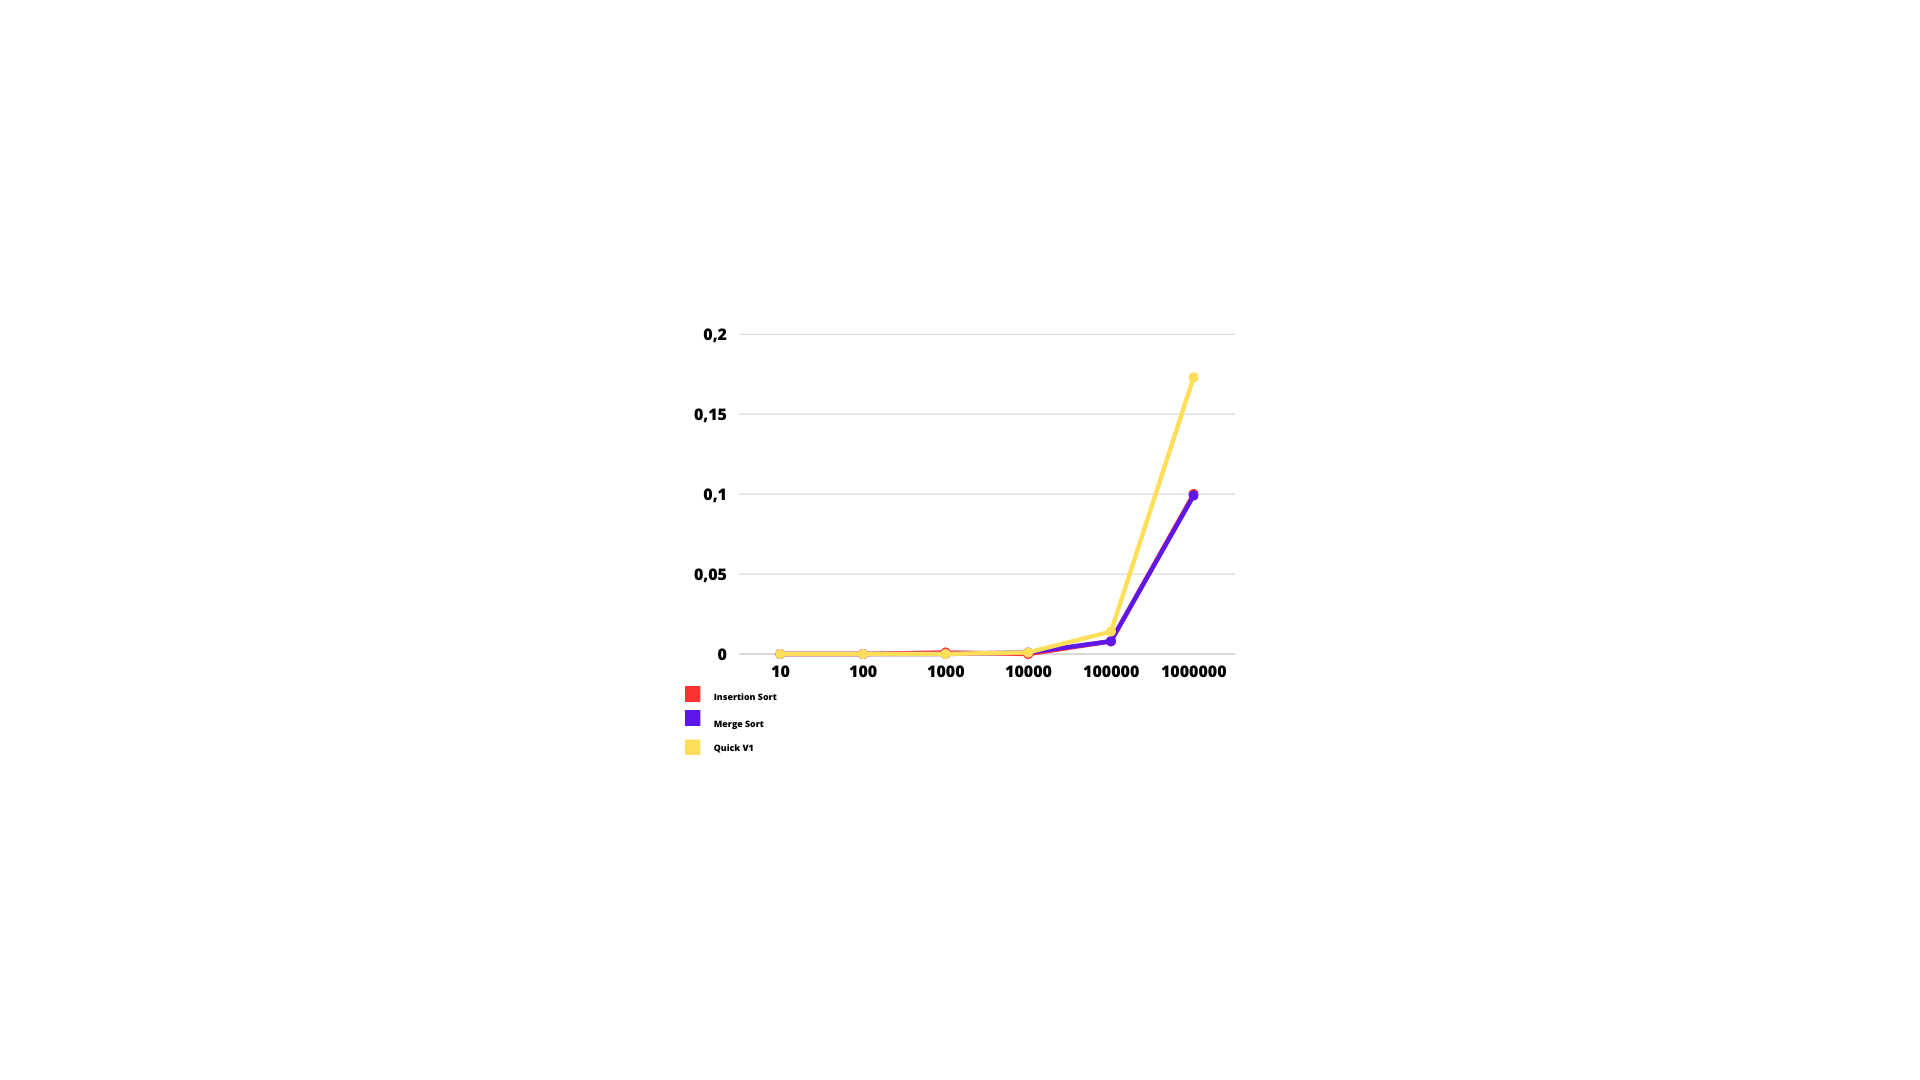
\includegraphics[width = 20cm]{Imagens/Merge Sort/merge.png}
    \caption{Gráfico de tempo do Merge Sort. }
    \label{imagem_digrama}
\end{figure}


